\section{Clustering}
\subsection{Unsupervised Learning}
\begin{itemize}
    \item We are given Data (features, x) wihout labels (y)
    \item Can we still learn something from the data?
    \item Yes! Often the data has some structure
    \item \textbf{The goal} of unsupervised learning is to self-discover patterns from the data
\end{itemize}

\subsection{Clusters}
\begin{itemize}
    \item Data points which have shared properties
    \item Fall into one cluster or one alike group
    \item Similar Data Points are close together
\end{itemize}
\subsubsection{Applications}
\begin{itemize}
    \item Social Network Analysis
    \item Astronomical Data
    \item Marked segmentation
    \item Recommendation systems
\end{itemize}
\subsection{Naive K-means}
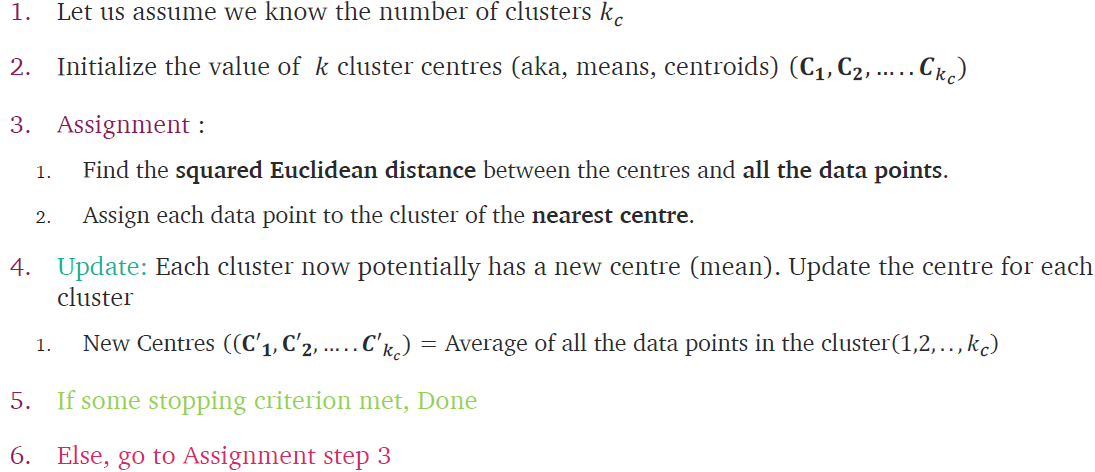
\includegraphics[width=\linewidth]{./img/k-means.png}

\subsubsection{Stopping Criterion}
\begin{itemize}
    \item When centres don't change (time consuming)
    \item The datapoints assigned to specific cluster remains the same (takes too much time)
    \item The distance of datapoints from their centres $>=$ treshold we have set
    \item Fixed number of iterations have reached (choose wisely)
\end{itemize}

\subsubsection{Initialization}
\begin{itemize}
    \item Performance depends on the random initialization
    \item Some seeds can result in a poor convergence rate
    \item Some seeds can converge to suboptimal clustering
    \item If centres are very close, it takes a lot of iterations to converge
    \item Initialize randomly, run multiple times
\end{itemize}

\subsubsection{Standardization of data}
\begin{itemize}
    \item Features with large values may dominate the distance value
    \item Features over small values will have no impact
    \item Normalize values!
\end{itemize}

\subsubsection{Sklean k-means}
\textbf{Initialization}
\begin{itemize}
    \item Init = K-means++
    \item Only initialization of the centroids will change
    \item Chosen centroids should be far from each other
\end{itemize}
\textbf{max\_iter:}
\begin{itemize}
    \item Number of iterations before stopping
\end{itemize}
\textbf{n\_init:}
\begin{itemize}
    \item Number of time the k-means algorithm will be run with different centroid seeds
\end{itemize}

\subsubsection{Evaluating Cluster Quality}
\begin{itemize}
    \item Make clusters so that for each cluster the distance of each cluster member from its center is minimizes
\end{itemize}
\textbf{Inertia or within-cluster sum-of-squares (WCSS)}
\begin{itemize}
    \item Sum of squared distances to center
    \item As small as possible
\end{itemize}
\textbf{Silhouette Score}
\begin{itemize}
    \item How far the datapoints in one cluster are from the datapoints in another cluster
    \item SS of a point: $\frac{b-a}{max(a,b)}$
    \item a: average intra-cluster distance (distance between each point within)
    \item b: average inter-cluster distance (distance between a cluster and its nearest neighbour)
\end{itemize}